% CSML Independent Work Poster -- 36" x 24" landscape
% Compile: pdflatex poster.tex
\documentclass[10pt]{article}

\usepackage{fix-cm}
\usepackage[paperwidth=36in,paperheight=24in,margin=0.42in]{geometry}
\usepackage{xcolor}
\usepackage{graphicx}
\usepackage{booktabs}
\usepackage{amsmath,amssymb}
\usepackage{multicol}
\usepackage{microtype}
\usepackage{enumitem}
\usepackage{hyperref}

\pagestyle{empty}
\setlength{\parindent}{0pt}
\setlength{\parskip}{3pt}
\setlength{\columnsep}{0.38in}
\setlist[itemize]{leftmargin=0.9em,itemsep=2pt,topsep=2pt}

\definecolor{princetonOrange}{HTML}{E77500}
\definecolor{ink}{HTML}{111111}
\definecolor{slate}{HTML}{233142}
\definecolor{softBlue}{HTML}{EAF2F8}
\definecolor{softOrange}{HTML}{FFF0DF}
\definecolor{softGreen}{HTML}{EAF6EF}
\definecolor{ruleGray}{HTML}{CDD5DF}

\newcommand{\panel}[2]{%
  \noindent\fcolorbox{ruleGray}{#1}{%
    \begin{minipage}{\dimexpr\linewidth-2\fboxsep-2\fboxrule\relax}
    \vspace{0.10in}
    #2
    \vspace{0.10in}
    \end{minipage}}%
  \par\vspace{0.13in}}

\newcommand{\paneltitle}[1]{%
  {\fontsize{27}{30}\selectfont\bfseries\color{slate} #1}\par
  \vspace{3pt}{\color{princetonOrange}\rule{\linewidth}{2pt}}\vspace{5pt}}

\begin{document}

\begin{center}
{\fontsize{56}{62}\selectfont\bfseries\color{ink} Polynomial Input Preconditioning for Zero-Shot Time-Series Forecasting}\par
\vspace{0.08in}
{\fontsize{24}{28}\selectfont Jerry Han \quad | \quad Advisor: Prof. Elad Hazan \quad | \quad Program in Statistics and Machine Learning, Princeton University}\par
\vspace{0.08in}
{\color{princetonOrange}\rule{\linewidth}{4pt}}
\end{center}

\vspace{0.15in}

\begin{multicols}{3}

\panel{softBlue}{
\paneltitle{Problem}
{\fontsize{17}{21}\selectfont
Patch-based time-series transformers embed each patch independently before attention. This is efficient, but it means each initial token only sees its local $P$-step window. Long-range structure across patches has to be discovered entirely inside the transformer.

\vspace{0.06in}
\textbf{Research question:} can a fixed polynomial transformation expose useful cross-patch structure before tokenization?
}
}

\panel{softGreen}{
\paneltitle{Preliminaries}
{\fontsize{16}{20}\selectfont
Universal Sequence Preconditioning preprocesses a sequence with a fixed polynomial convolution,
\[
x_t^{\mathrm{pre}}=\sum_{k=0}^{d}c_k x_{t-k}.
\]
In the online linear-dynamical-systems setting, this kind of transformation can improve regret bounds by reducing the effective difficulty of the hidden dynamics. This project tests whether the same idea helps in a different setting: offline pretraining and zero-shot multi-step forecasting.
}
}

\panel{softOrange}{
\paneltitle{Method}
{\fontsize{17}{21}\selectfont
For a normalized time series $x_t$, compute a fixed Chebyshev residual
\[
r_t=\sum_{k=1}^{d}c_k x_{t-ks}.
\]
With $d=4$ and stride $s=P=16$,
\[
r_t=-x_{t-32}+\frac{1}{8}x_{t-64}.
\]
Concatenate this as a third input channel:
\[
\mathbf e_i=\mathrm{ResBlock}_{3P\to d}([\mathbf p_i;\mathbf m_i;\mathbf r_i]).
\]
Only the input projection widens; the transformer decoder and forecasting target are unchanged.
}
}

\panel{softGreen}{
\paneltitle{Architecture}

\includegraphics[width=\linewidth]{figures/fig_architecture.pdf}
{\fontsize{14}{17}\selectfont
Orange components are the only changes relative to Moirai 2.0: preconditioning residual, optional training-time channel dropout, concatenation, and the widened input projection.
}
}

\columnbreak

\panel{softBlue}{
\paneltitle{Experimental Design}
{\fontsize{16}{20}\selectfont
\begin{itemize}
\item Model: Moirai 2.0 Small, 11.4M parameters.
\item Data: public LOTSA setup, 27B observations.
\item Main budget: 10K optimizer steps, 5 seeds.
\item Extended budget: 100K optimizer steps, 5 seeds.
\item Primary benchmark: GIFT-Eval, 97 dataset-by-horizon configurations.
\item External benchmark: FEV-Bench, 100 forecasting tasks.
\item Metric: geometric-mean MASE; lower is better.
\end{itemize}
}
}

\panel{softOrange}{
\paneltitle{Main Results}
{\fontsize{16}{20}\selectfont
The polynomial channel improves GIFT-Eval normalized MASE by $2.9\%$, wins 72 of 97 configurations after averaging across five seeds, adds only $0.11\%$ parameters, and reaches a $3.9\%$ improvement at 100K training steps.
}
\vspace{0.04in}
\begin{center}
\fontsize{15}{18}\selectfont
\begin{tabular}{lccc}
\toprule
Method & MASE & $\Delta$ & Wins \\
\midrule
\textbf{\texttt{d4\_dropout}} & \textbf{0.837} & \textbf{$-2.9\%$} & \textbf{72/97} \\
\texttt{d4} & 0.838 & $-2.8\%$ & 72/97 \\
Zero ctrl & 0.858 & $-0.5\%$ & 54/97 \\
Baseline & 0.862 & --- & --- \\
Duplicate ctrl & 0.865 & $+0.4\%$ & 39/97 \\
\bottomrule
\end{tabular}
\end{center}
{\fontsize{16}{20}\selectfont
The capacity-matched controls show the effect is not just from adding parameters. A zero channel is neutral, while duplicating the raw input hurts.
}
}

\panel{softGreen}{
\paneltitle{Statistical Evidence}
{\fontsize{17}{21}\selectfont
For GIFT-Eval, I average MASE per configuration across five seeds and run a two-sided paired sign test. \texttt{d4\_dropout} wins 72 of 97 configurations over the baseline, giving $p<10^{-5}$.

\vspace{0.05in}
This is a controlled paired comparison: every model is trained with the same data, optimizer, precision, and seed set within the compared condition.
}
}

\panel{softBlue}{
\paneltitle{Fixed vs. Learned Filters}
\begin{center}
\fontsize{14}{17}\selectfont
\begin{tabular}{lcc}
\toprule
Setting & MASE & $\Delta$ \\
\midrule
\textbf{Fixed Chebyshev} & \textbf{0.8234} & \textbf{$-4.99\%$} \\
Learned, Cheb. init & 0.8332 & $-3.85\%$ \\
Learned, zero init & 0.8358 & $-3.57\%$ \\
\bottomrule
\end{tabular}
\end{center}
{\fontsize{16}{20}\selectfont
The fixed Chebyshev coefficients outperform learned coefficient vectors, even when the learned model is initialized at Chebyshev. This suggests the polynomial channel is a useful inductive bias.
}
}

\panel{softOrange}{
\paneltitle{Personal Contribution}
{\fontsize{16}{20}\selectfont
\begin{itemize}
\item Implemented the preconditioning channel in the Moirai 2.0 training/evaluation pipeline.
\item Designed the zero and duplicate capacity controls.
\item Ran the seed, degree, coefficient-learning, horizon, and 100K-step analyses.
\item Prepared the CSML paper, poster, and presentation materials.
\item Thanks to Alex Kawaja for working together on this collaborative project.
\end{itemize}
}
}

\columnbreak

\panel{softBlue}{
\paneltitle{Ablations}
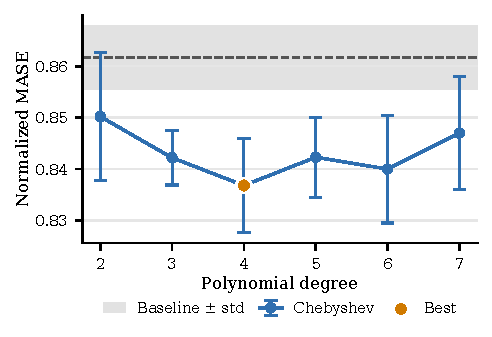
\includegraphics[width=0.92\linewidth]{figures/degree_sweep_line.pdf}\par
{\fontsize{15}{18}\selectfont
All tested Chebyshev degrees improve over baseline. Degree 4 is a strong default, not a sharply tuned optimum.
}
}

\panel{softOrange}{
\paneltitle{Independent Benchmark}
\begin{center}
\fontsize{15}{18}\selectfont
\begin{tabular}{lcc}
\toprule
Method & MASE & SQL \\
\midrule
\textbf{\texttt{d4\_dropout}} & \textbf{1.2532} & \textbf{1.0236} \\
Baseline & 1.2908 & 1.0562 \\
$\Delta$ & $-2.91\%$ & $-3.09\%$ \\
\bottomrule
\end{tabular}
\end{center}
{\fontsize{16}{20}\selectfont
The improvement transfers to FEV-Bench, an independent benchmark with 100 forecasting tasks from 96 datasets.
}
}

\panel{softBlue}{
\paneltitle{Horizon Effects}
\begin{center}
\fontsize{14}{17}\selectfont
\begin{tabular}{lccc}
\toprule
Term & Baseline & \texttt{d4} & \texttt{d4\_dropout} \\
\midrule
Short & 0.840 & \textbf{0.825} & 0.828 \\
Medium & 0.859 & 0.830 & \textbf{0.823} \\
Long & 0.924 & 0.880 & \textbf{0.874} \\
\bottomrule
\end{tabular}
\end{center}
{\fontsize{15}{18}\selectfont
The largest gain is on long-horizon tasks: \texttt{d4\_dropout} improves MASE by $5.3\%$ relative to baseline in the long-horizon bin.
}
}

\panel{softGreen}{
\paneltitle{Training Dynamics}
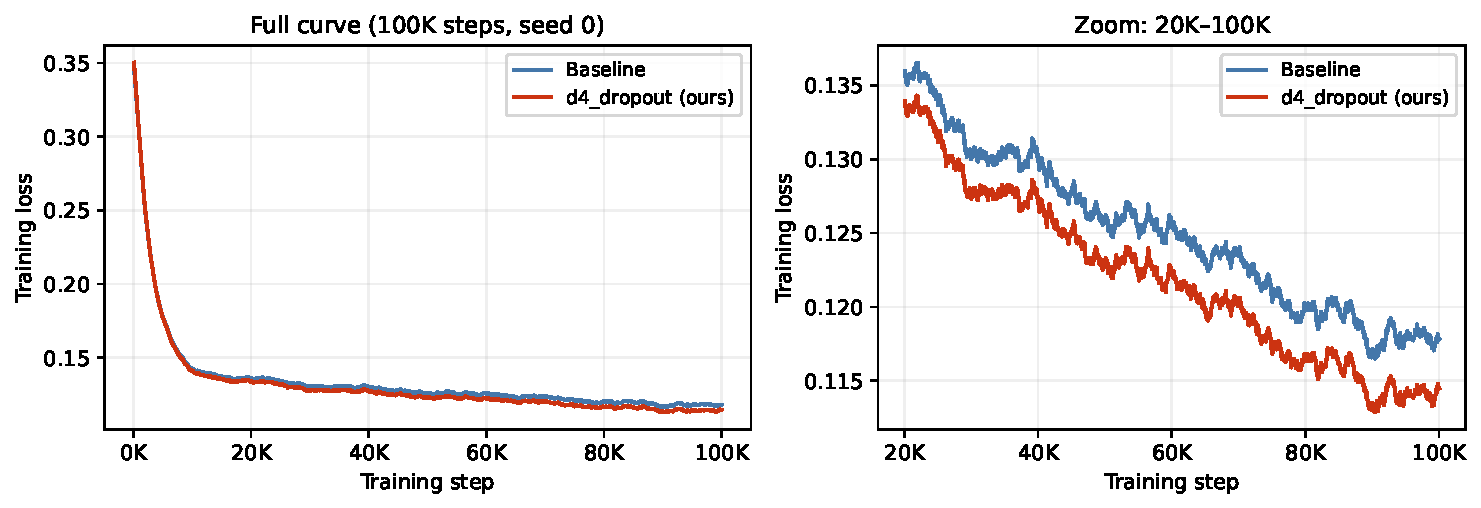
\includegraphics[width=\linewidth]{figures/fig_training_loss_main.pdf}
{\fontsize{15}{18}\selectfont
At 100K training steps, the MASE improvement grows to $-3.9\%$. The preconditioned model also has lower cross-seed standard deviation: 0.0079 vs 0.0189 for the baseline.
}
}

\end{multicols}

\vspace{0.03in}
\noindent\fcolorbox{princetonOrange}{white}{%
\begin{minipage}{\dimexpr\linewidth-2\fboxsep-2\fboxrule\relax}
\vspace{0.08in}
{\fontsize{24}{28}\selectfont\bfseries\color{slate} Takeaway:}
{\fontsize{21}{25}\selectfont
 A fixed, theory-guided input channel improves a modern time-series foundation model without changing the transformer stack. The gain comes from polynomial content, not added width, and is strongest at longer training budgets and longer horizons.}
\vspace{0.08in}
\end{minipage}}

\vfill
\begin{center}
{\fontsize{13}{16}\selectfont
CSML Independent Work, Spring 2026 \quad | \quad Code and paper repository: \url{https://github.com/jerryhan60/ts-usp-paper} \quad | \quad Contact: \texttt{jh1161@princeton.edu}}
\end{center}

\end{document}
